\documentclass[aspectratio=169,xcolor=dvipsnames]{beamer}
\usepackage{comp2402}

\title{Interfaces/Abstract Data Types}
\author{COMP2402}
\date{}

\begin{document}

\begin{frame}
  \titlepage
\end{frame}

\begin{frame}
  \frametitle{Interfaces/Abstract Data Types}
 
  \begin{itemize}
   \item<+->Describes what a data structure \emph{does}:
     \begin{itemize}
        \item<+->supported operations (the \emph{interface})
        \item<+->meaning of operations (the \emph{semantics})
     \end{itemize}
   \item<+-> \sout{Representation and implementation}
        \end{itemize}
\end{frame}

\begin{frame}
  \frametitle{Abstract Data Types/Interfaces}

  \begin{tabular}{p{.3\textwidth}p{.6\textwidth}}
  \raisebox{-.5\height}{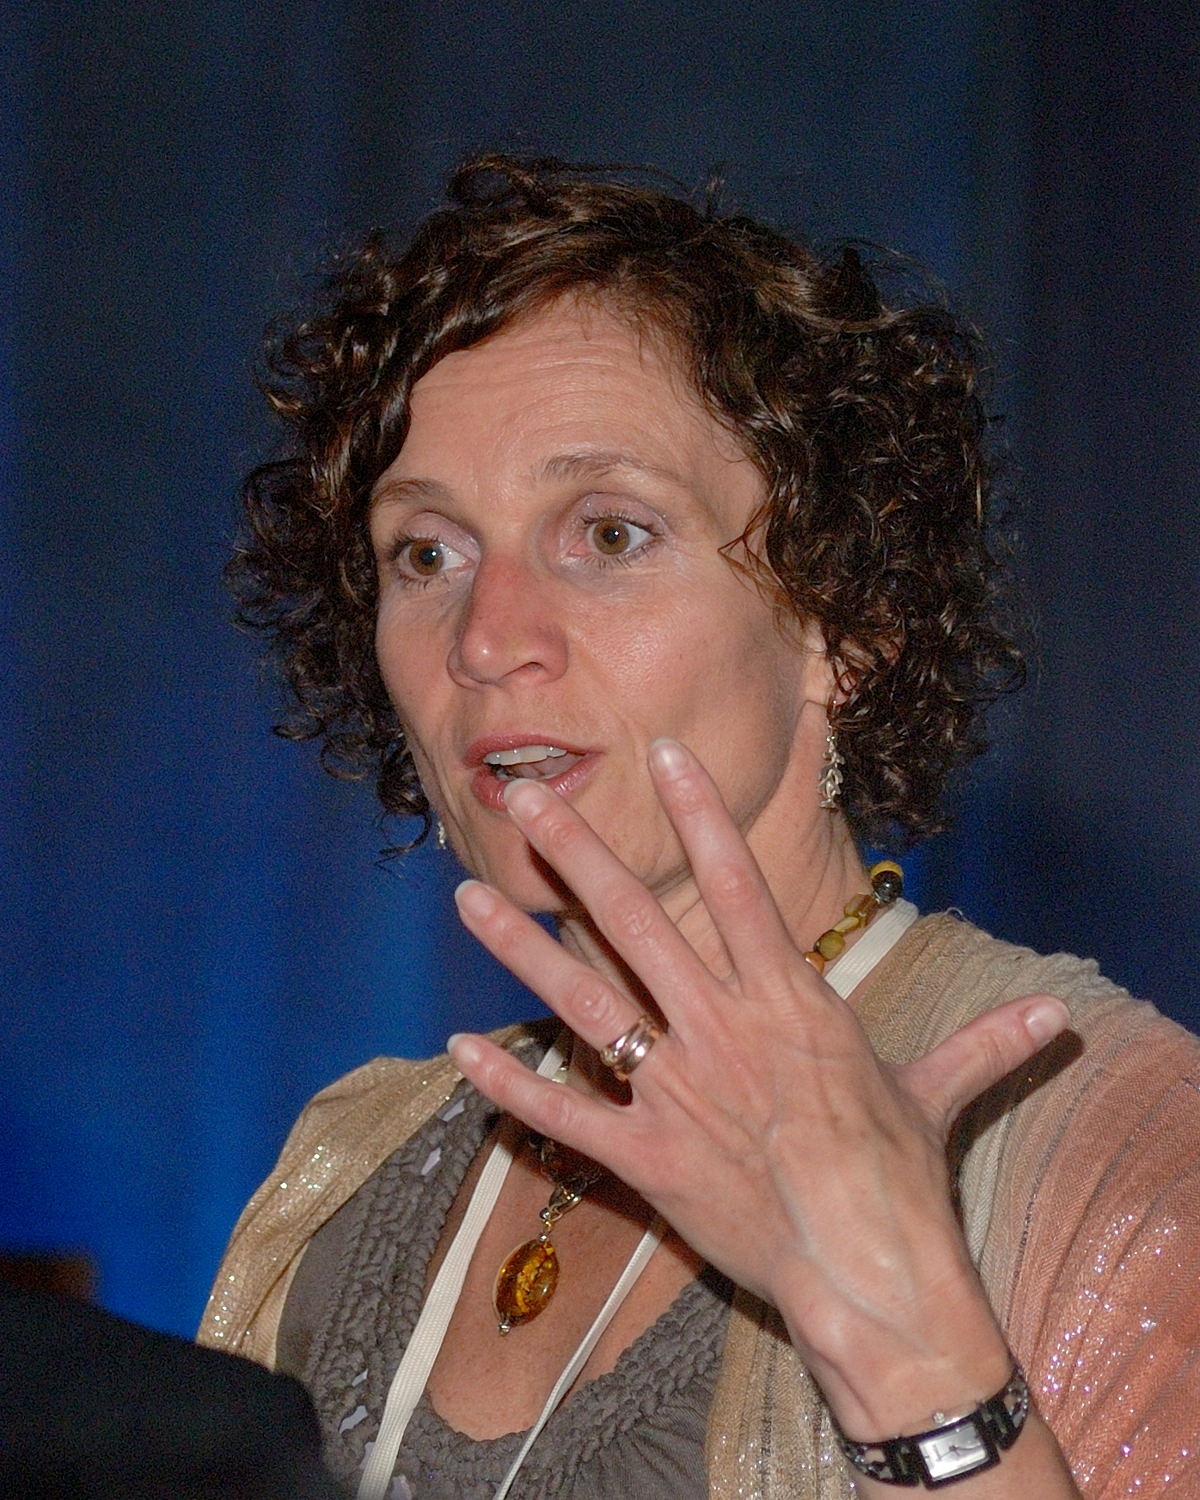
\includegraphics[width=.28\textwidth]{images/liskov}} \newline\newline
  \raggedright   Barbara Liskov at the ACM Turing Centenary Celebration
  \mbox{(\copyright~2012~Dennis~Hamilton)}
 &

   \raggedright B. Liskov and S. N. Zilles, Programming with Abstract Data Types, \emphen{SIGPlan Notices}, 9(4), pp. 50-59, 1974.\\
  \end{tabular}
\end{frame}

\titler{The List Interface}


\begin{frame}
  \frametitle{List}
  \framesubtitle{A sequence of elements}
 
  \begin{itemize}
    \item<+(2)-> Operations: \only<+(2)->{#get(i)#}%
                        \only<+(2)->{, #set(i,x)#}%
                        \only<+(2)->{, #add(i,x)#}%
                        \only<+(2)->{, #remove(x)#}
  \end{itemize}
     \begin{center}
      \only<1>{\includegraphics{figs/list-1}}%
      \only<2-7>{\includegraphics{figs/list-2}}%
      \only<8->{\multiinclude[<+>][format=pdf,start=4]{figs/list}}
     \end{center}
\end{frame}


\titler{The USet (Unordered Set) Interface}


\begin{frame}
  \frametitle{USet}
  \framesubtitle{An \emphen{unordered} collection of \emphen{distinct} items}
  \begin{itemize}
    \item<+-> Operations: \only<+->{#add(x)#}%
                        \only<+->{, #remove(x)#}%
                        \only<+->{, #find(x)#}%
  \end{itemize}
     \begin{center}
      \only<1-4>{\includegraphics{figs/uset-1}}%
      \only<5->{\multiinclude[<+>][format=pdf,start=1]{figs/uset}}
     \end{center}

\end{frame}

\begin{frame}
  \frametitle{Map}
  \framesubtitle{A #USet# that stores key/value pairs}
 
     \begin{center}
      \multiinclude[<+>][format=pdf,start=1]{figs/map}
     \end{center}
\end{frame}

\titler{The SSet (Sorted Set) Interface}

\begin{frame}
  \frametitle{SSet}
  \framesubtitle{A Sorted Set}
 
  \begin{itemize}
    \item<+->Stores \emph{comparable} items
    \begin{itemize}
       \item<+-> Numbers: $0 < 1 < 2 < 3 < \cdots < 4294967296$
       \item<+-> Letters: $a < b < c < d < \cdots < z$
       \item<+-> Strings: $\text{``apple''} < \text{``bread''} < \text{``brie''} 
                           < \text{``cheese''} < \cdots < \text{``zyxt''}$
    \end{itemize}
  \end{itemize}
\end{frame}

\begin{frame}
  \frametitle{SSet}
  \framesubtitle{A Sorted Set}

  \begin{itemize}
    \item<+-> Operations: \only<+->{#add(x)#}%
                        \only<+->{, #remove(x)#}%
                        \only<+->{, #find(x)#}%
  \end{itemize}
  \begin{center}
      \only<1-4>{\includegraphics{figs/sset-1}}%
      \only<5->{\multiinclude[<+>][format=pdf,start=1]{figs/sset}}
  \end{center}
\end{frame}

\titler{}



\end{document}

